\begin{example}
    \begin{figure}
        \centering
        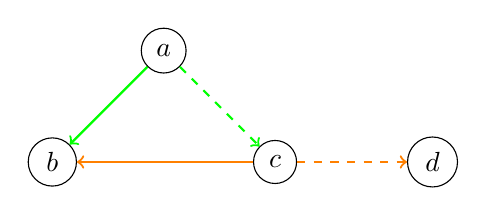
\begin{tikzpicture}[
                node distance={20mm},
                main/.style = {draw, circle},
                s/.style = {->,thick},
                d/.style = {->,thick,dashed} ]
            \node[main] (b) {$b$};
            \node[main] (a) [above right of=b] {$a$};
            \node[main] (c) [below right of=a] {$c$};
            \node[main] (d) [right of=c] {$d$};
            \draw[thick,green,->] (a) -- (b);
            \draw[thick,green,->,dashed] (a) -- (c);
            \draw[thick,orange,->] (c) -- (b);
            \draw[thick,orange,->,dashed] (c) -- (d);
        \end{tikzpicture}
        \caption{}
        \label{fig:blacklist}
    \end{figure}
    Blacklisted nodes are nodes in the network that must not
    be reachable \cite{network-abstractions}.
    Let's assume the network in figure \ref{fig:blacklist} as
    an example where the node $d$ is blacklisted.
    For simplicity we assume that we require
    $d$ not reachable only from $a$.
    Consider the following DyNetKAT program for this network:
    \begin{equation*}
        \begin{aligned}[c]
            P   & = p!1                             \\
            Q   & = q!1                             \\
            N   & = F \oplus p?1;N_p \oplus q?1;N_q \\
            N_p & = F_p \oplus q?1;F_{pq}           \\
            N_q & = F_q \oplus p?1;F_{pq}           \\
            F   & = a\ra b \oplus c\ra b            \\
        \end{aligned}
        \qquad\qquad
        \begin{aligned}[c]
            F_p         & = a\ra c \oplus c\ra b \oplus a\ra b \\
            F_q         & = a\ra b \oplus c\ra d               \\
            F_{pq}      & = a\ra c \oplus c\ra d \oplus a\ra d \\
            SDN         & = \delta_{\mathcal{L}} (N
            \parallel P \parallel Q)                           \\
            \mathcal{L} & = \s{p!1,p?1,q?1,q?1}                \\
        \end{aligned}
    \end{equation*}
    We assume that there are two concurrent processes for updating
    the switches $a$ and $c$.
    Let we use $p$ and $q$ to denote $rcfg(p,1)$ and
    $rcfg(q,1)$ respectively.
    Thus, $p$ and $q$ replace the solid green and orange
    paths in the network with dashed paths respectively.
    \begin{figure}
        \centering
        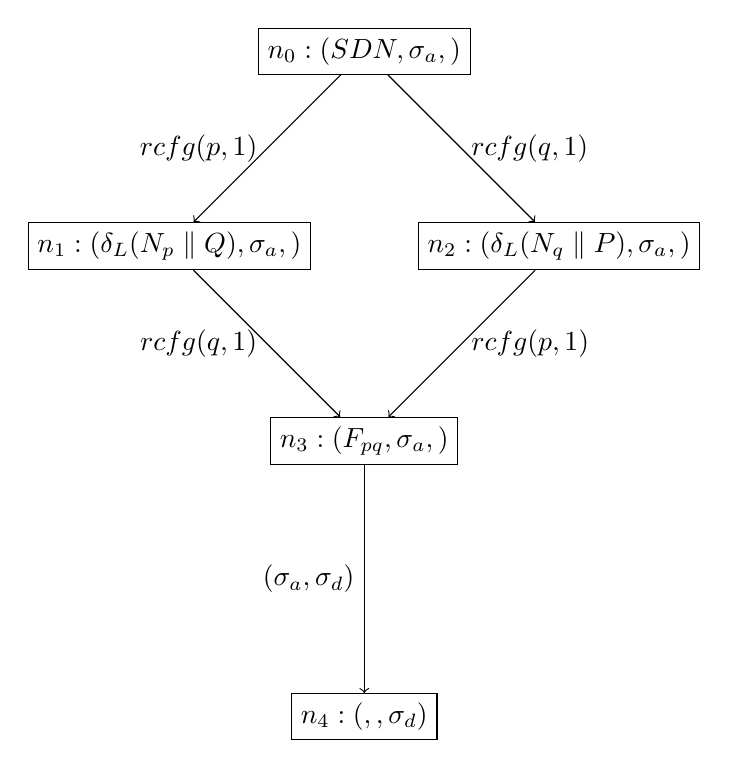
\begin{tikzpicture}[node distance={35mm},
                s/.style = {draw, rectangle,minimum width=5mm} ]
            \node[s] (n0) {$n_0: (SDN,\sigma_a,\his{})$};
            \node[s] (n1) [below left of=n0]
            {$n_1: (\delta_{\mc{L}}(N_p \parallel Q),\sigma_a,\his{})$};
            \node[s] (n3) [below right of=n1]
            {$n_3: (F_{pq},\sigma_a,\his{})$};
            \node[s] (n4) [below of=n3]
            {$n_4:(\checkmark,\his{},\sigma_d)$};
            \node[s] (n2) [below right of=n0]
            {$n_2: (\delta_{\mc{L}}(N_q \parallel P),\sigma_a,\his{}$)};
            \draw[->] (n0) -- node[left]{$rcfg(p,1)$} (n1);
            \draw[->] (n0) -- node[right]{$rcfg(q,1)$} (n2);
            \draw[->] (n1) -- node[left]{$rcfg(q,1)$} (n3);
            \draw[->] (n2) -- node[right]{$rcfg(p,1)$} (n3);
            \draw[->] (n3) -- node[left]{$(\sigma_a,\sigma_d)$} (n4);
        \end{tikzpicture}
        \caption{}
        \label{fig:blacklist:lts}
    \end{figure}
    Figure \ref{fig:blacklist:lts} shows an excerpt of the LTS of $SDN$ 
    when there is a packet $\sigma_a$ where $\sigma_a(sw) = a$.
    Obviously, executing both $rcfg_{p,1}$ and $rcfg_{q,1}$ leads
    to a state where we can forward the $\sigma_a$ to $d$.
    To find the cause of error, let $\mr{E} = \sem{SDN}$ and $\mc{M}$ 
    be the causal model of $\mr{E}$ where we encoded the unsafe behavior 
    as:
    \begin{equation*}
        \f{PV} = \exists c \in \mc{F}(ES(\vec v)). \exists e \in c. l(e) = a\ra d
    \end{equation*}
    The function above sets the value of $PV$ to true if $ES(\vec v)$ 
    contains a configuration with an event labeled $a \ra d$.
    In $SDN$ there are two order execution for $p$ and $q$ so,
    there are two events for each of these labels in $\mr{E}$ 
    and thus, there are two events with the label $a \ra b$ as well.
    So, let's consider events $p_1,p_2$ with label $p$,
    events $q_1,q_2$ with label $q$ and events $ad_1,ad_2$ 
    with label $a \ra d$ in $E$.
    \begin{figure}
        \centering
        \begin{tikzpicture}
            \crd{0}{0}{$\emptyset$}
            \crd[left]{-2}{1}{$\s{p_1}$}
            \crd[left]{-2}{2}{$\s{p_1,q_1}$}
            \crd[left]{-2}{3}{$\s{p_1,q_1,ad_1}$}
            \crd[right]{2}{1}{$\s{q_2}$}
            \crd[right]{2}{2}{$\s{p_2,q_2}$}
            \crd[right]{2}{3}{$\s{p_2,q_2,ad_2}$}
            \draw [ultra thick] (-2,1) -- (-2,2);
            \draw [ultra thick] (-2,2) -- (-2,3);
            \draw [ultra thick] (0,0) -- (2,1);
            \draw [ultra thick] (0,0) -- (-2,1);
            \draw [ultra thick] (2,1) -- (2,2);
            \draw [ultra thick] (2,1) -- (2,3);
        \end{tikzpicture}
        \caption{}
        \label{fig:blacklist:es}
    \end{figure}
    Figure \ref{fig:blacklist:es} shows a portion of $\mr{E}$ consist of
    configurations leading to events labeled with $a\ra d$.

    In this example we can consider $C_{p_1,q_2} = \F$ as a cause of 
    $PV = \T$ using the witness $(C_{p_2,q_2},\T,\T)$.
    Let $\vec v'$ be the values of variables when we set both 
    $C_{p_1,q_1}$ and $C_{p_2,q_2}$ to $\T$.
    Thus we have:
    \begin{equation*}
        \mc{M} \vDash [C_{p_1,q_1} \la \T, C_{p_2,q_2} \la T] 
        \vec V = \vec v'
    \end{equation*}
    Obviously, neither $\s{p_1,q_1,ad_1}$ nor $\s{p_2,q_2,ad_2}$ 
    are not configurations of $ES(\vec v')$ because we have
    $p_1 \# q_1$ and $p_2 \# q_2$.
    So, we can claim that:
    \begin{equation*}
        \mc{M} \vDash [C_{p_1,q_1} \la \T, C_{p_2,q_2} \la T] 
        PV = \F
    \end{equation*}
    Which satisfies the AC2.a condition.

    Now, for the AC2.b condition, we need to consider contingencies 
    where we set $C_{p_1,q_1}$ to $\F$, $C_{p_2,q_2}$ to $\T$ and 
    resetting values of any subset of other variables to their 
    original values.
    If we set $C_{p_1,q_1}$ to $\F$ it means that we removed
    the conflict between $p_1$ and $q_1$ so $\s{p_1,q_1,ad_1}$ becomes
    a configuration of the $ES(\vec v)$ again.
    Note that value of $C_{p_2,q_2}$ has no effect on this.
    Formally, this means that:
    \begin{equation*}
        \mc{M} \vDash [C_{p_1,q_1} \la \F, C_{p_2,q_2} \la T
            ,\vec Z' \la \vec z^*
        ] \vec V = \vec v \wedge 
        (\vec v \in \mc{E} \Rightarrow PV = \T)
    \end{equation*}
    Thus, we can conclude that the AC2.b condition is also satisfied 
    and since the cause is a single conjunct the AC3 condition is
    satisfied too.
    So, we can conclude that the lack of conflict between $p_1$ and 
    $q_1$ is an actual of the property violation. 


\end{example}